\section{Design}
\label{sec:Design}

\subsection{Database Design} 
\paragraph{}The Bmob online database was chosen for the database management system (DBMS) for both the Android application and the web interface because it is a free and open source product that supports the application's required use-cases. 
\par The Bmob cloud storage service platform is a secure and flexible background management system which supports web-based database services, functions as a service (FaaS). In this application we will only use online database services. The Bmob cloud storage service platform adopts a multi-tenant virtual isolation mode, that is, any developer's traffic changes or data changes will not affect other developers' applications. 
Another reason to choose Bmob is it supports a well-designed REST API interface and multi-language SDK, with bindings for Java, IOS, JavaScript, GO and others as well. For our project, we will use the Java API and also make raw REST API calls using JQuery. It supports file uploads and storage,including pictures, videos, audio, and documents. CDN acceleration also makes the upload process faster and more stable but we will mainly use it to upload image files in this project. 
\par The entity relationship (ER) diagram for the whole project is shown in Figure \ref{ERDiagram}.

\begin{figure}[htb]
\centering
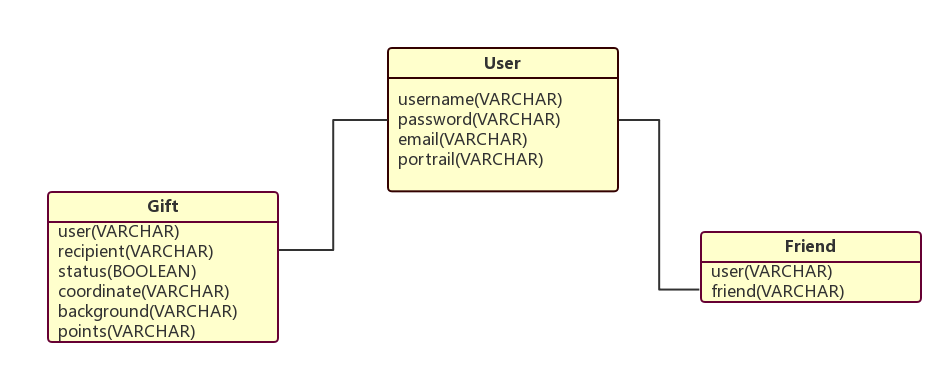
\includegraphics[width=1\textwidth]{section03/assets/ERDiagram.png}
\caption[ER Diagram for the project]{\label{ERDiagram}ER Diagram for the project}
\end{figure}


\begin{itemize}
\item The \bsq{User} table will save all the user information. In this table username and email will be unique for each user and users will receive an email after they registered.
\item The \bsq{Friend} table is for saving all friends pairs and both \bsq{user} and \bsq{friend} columns are usernames from \bsq{User} table.
\item The \bsq{Gift} table saves all the gifts information. The \bsq{user} column records the user who sent the gift. The \bsq{recipient} column records the user who will receive the gift. The \bsq{status} column is a Boolean type data meaning the gift is found if it is \bsq{true}. The \bsq{coordinate} column is designed to hold the location where the gift was sent. The \bsq{background} column is designed to hold the region picture. The \bsq{points} column is a string designed to hold the four corners selected by users, it has eight numbers separated by space which means four Xs and four Ys like (x1,y1),(x2,y2) will be saved as \bsq{x1 y1 x2 y2}.
\end{itemize}

\subsection{User Interface Design}
\paragraph{} We will have two parts for the user interface, one is about the Android application, the other one is for web interface.
\par Following user interface design principles, like accessibility, flexibility, consistency and aesthetics, this user interface is designed to be clear and easy to use. All pages keep the same color style and use limited colors and fonts so that the user interface is aesthetically pleasing.\cite{galitz2007} This section describes the main pages for both the Android and web application.
\subsubsection{Android Application User Interface Design}
\textbf{Sign In Page}
\par The sign in page is shown in Figure \ref{SignInUI}. The logo informs users which application they are using. The user icon and the password icon at the left side of the text field hint at the meaning of the two fields to the users. To maintain compatibility, the delete icon and the eye icon at the right side of the text field used another color because they have different functions. Users can use the delete button to clear the text field and use the eye button to view the password in plain text or hidden text.
\begin{figure}[H]
\centering
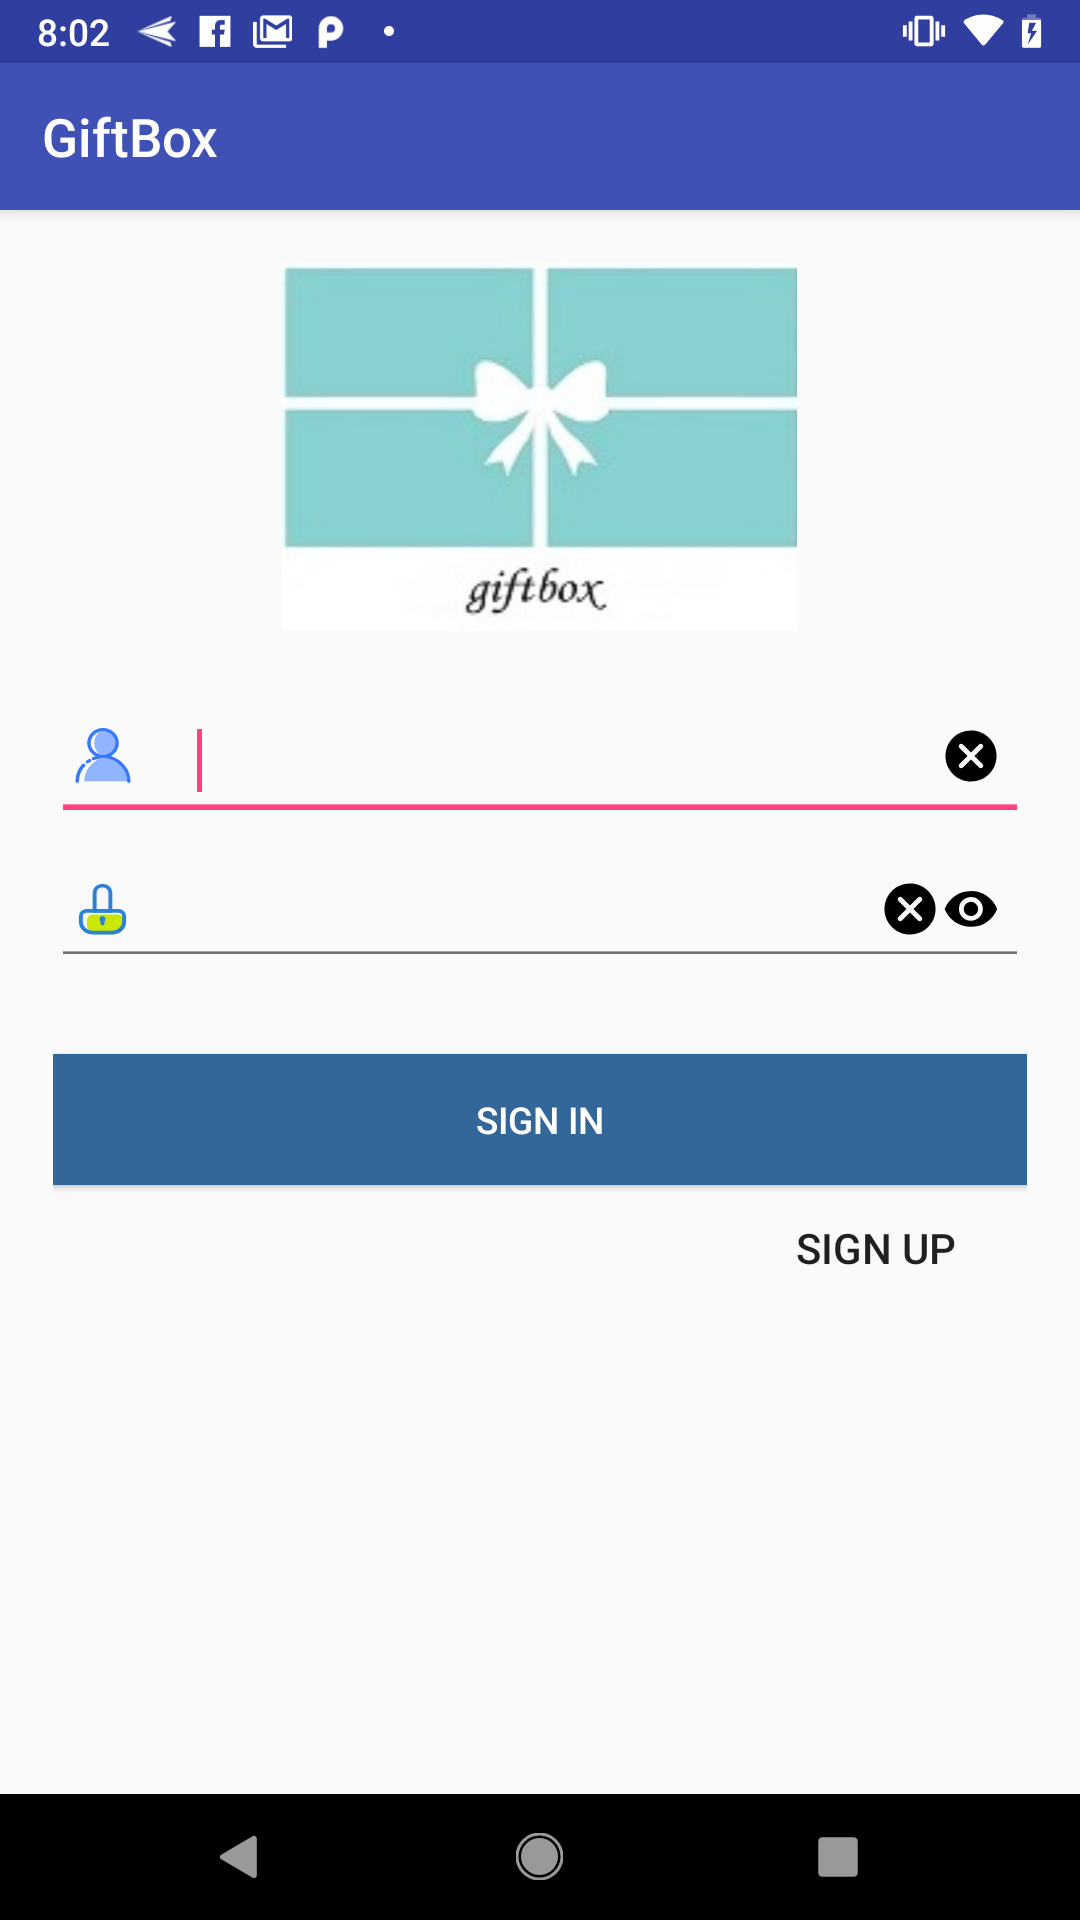
\includegraphics[width=.45\textwidth]{section03/assets/SignIn.png}
\caption[Sign In Page]{\label{SignInUI}Sign In Page}
\end{figure}

\textbf{Main Page}
\par The main page shown in Figure \ref{MainPageUI} will come up after users log in. The main page shows the gifts received by the user. The search field allows users to search for gifts by the username of the sender. The \bsq{found} column shows whether or not the gift has been found. If the \bsq{found} column is checked this means the gift has been found.
\par The top left corner navigation menu will lead users to other functional pages. Users will see their portrait on the top of this page and will be able to change their portrait by clicking on the portrait itself. They can also view their gifts list by clicking on the \bsq{Gifts} button, edit their profile by clicking on the \bsq{Edit Profile} button, view their friends list as shown in Figure \ref{FriendsListUI} by clicking on the \bsq{Friends} button and they will be able to log out from the system by clicking on the \bsq{LogOut} button. 

\begin{figure}[htb]
\centering
\begin{minipage}[t]{0.45\textwidth}
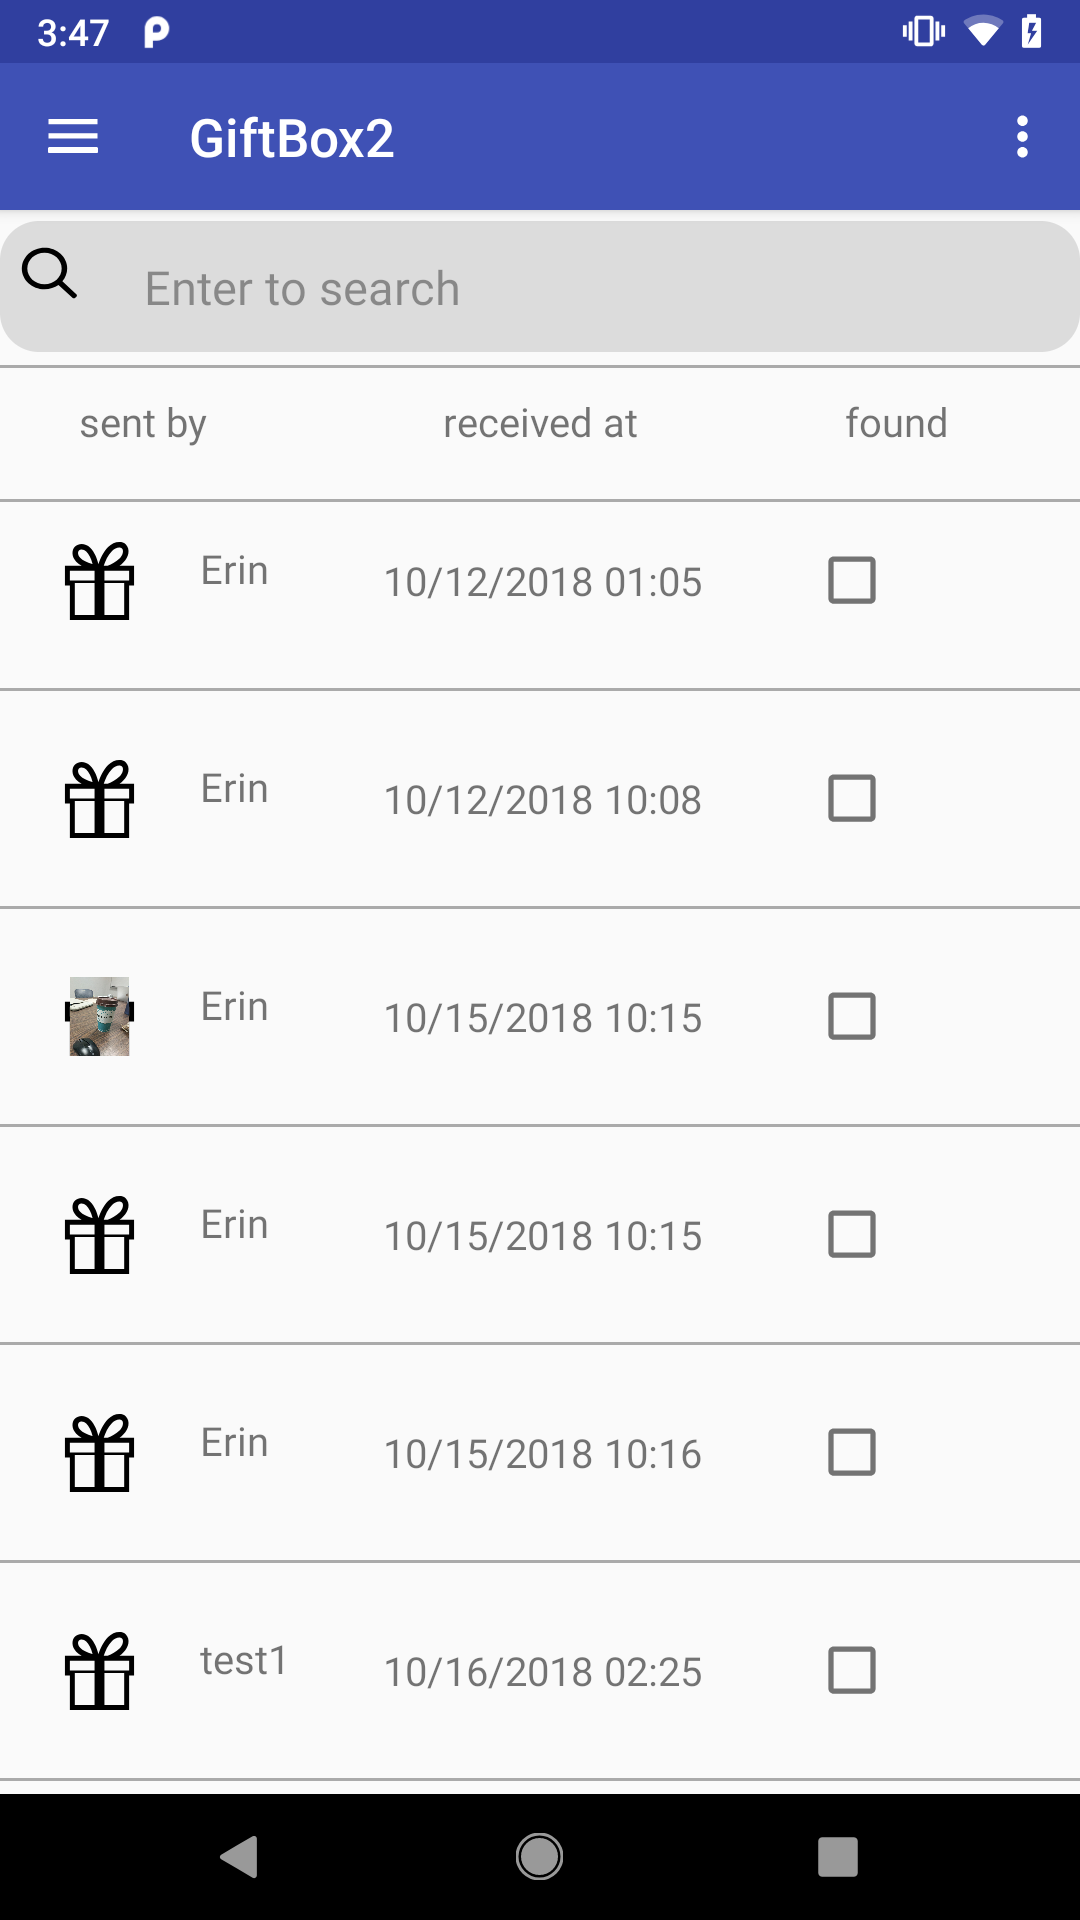
\includegraphics[width=.95\textwidth]{section03/assets/MainPage.png}
\subcaption{\label{GiftsListMainUI}}
\end{minipage}%
\begin{minipage}[t]{0.45\textwidth}
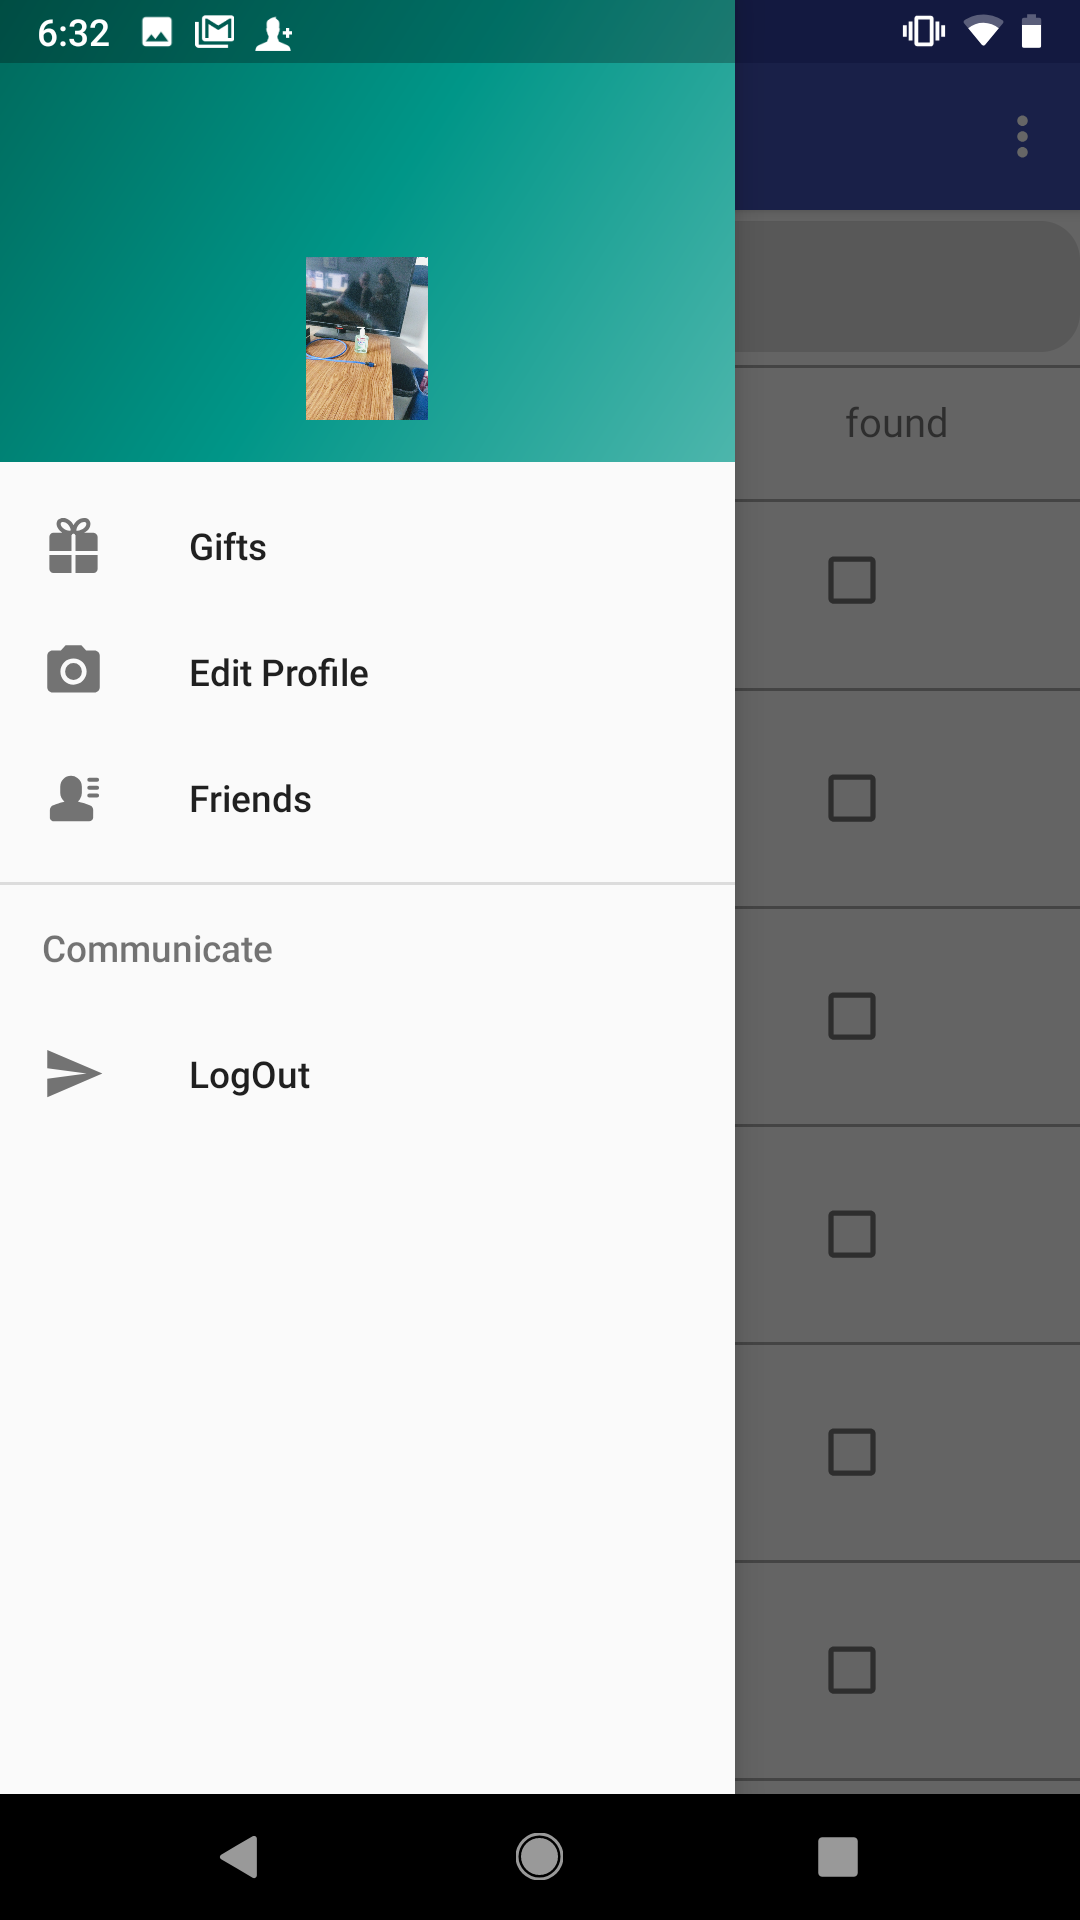
\includegraphics[width=.95\textwidth]{section03/assets/MainPortrait.png}
\subcaption{\label{FunctionsMainUI}}
\end{minipage}%
\caption[Main Page]{\label{MainPageUI}Main Page}
\end{figure}

\textbf{Gifts List Page}

\par Figure \ref{GiftsListUI} shows the \bsq{gifts list} which is very similar to the main page's gifts list but in this page users will be able to see not only their received gifts but also the gifts that they have sent ordered by time stamp. For the sent gifts, users will be able to see if the gift has been received and can view the gift details by clicking on the gift row. For gifts that they have received and found, clicking on the gift row will allow them to view the gift details.  For gifts that they have received but not found, they can begin to find these gifts by clicking on the gift row. 

\begin{figure}[htb]
\centering
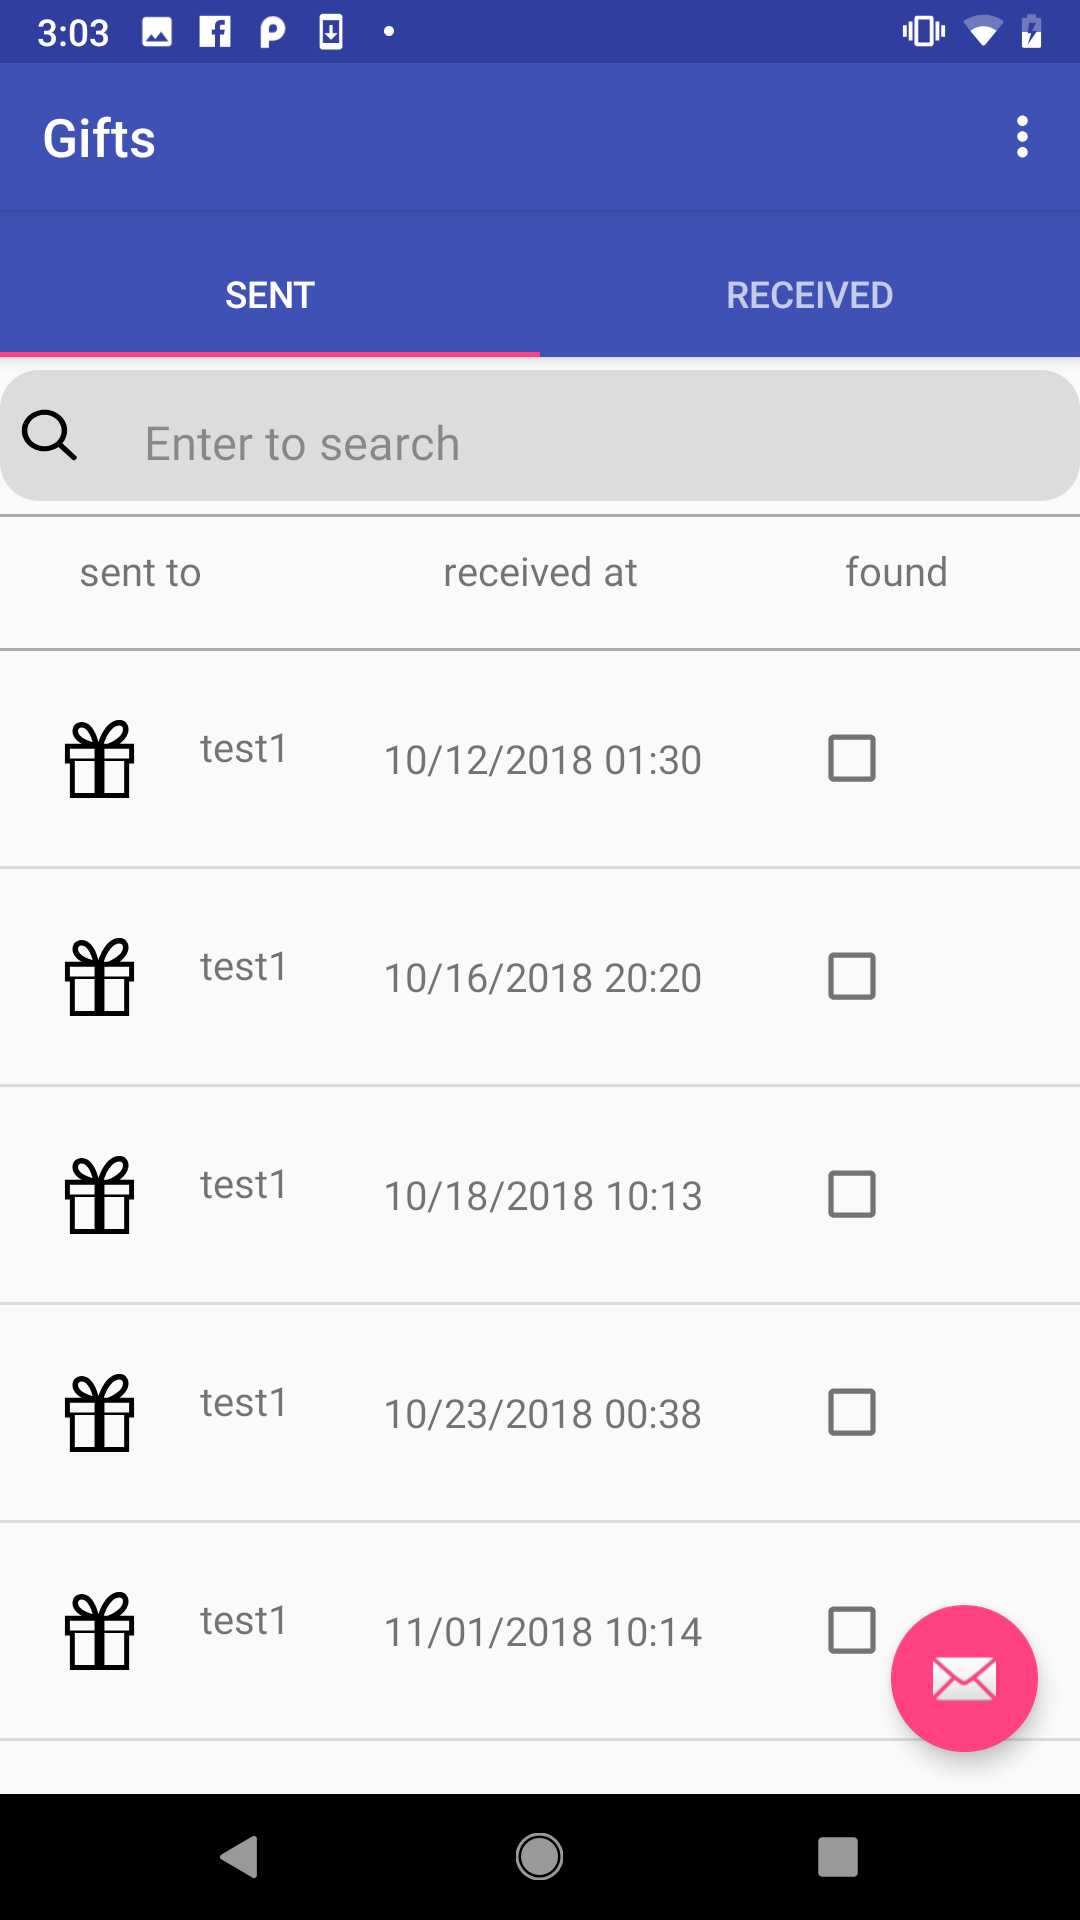
\includegraphics[width=.45\textwidth]{section03/assets/GiftsList.png}
\caption[Gifts List Page]{\label{GiftsListUI}Gifts List Page}
\end{figure}

\textbf{Friends List Page}

\par As shown in Figure \ref{WholeFriendsListUI}, the friends list is another important page for this application. For convenience, the search field allows users to search their list of friends if their friends list is too long. Users can also add friends by clicking on the \bsq{Add Friends} button. The friends list is shown below the \bsq{Add Friends} button. Users are able to send a gift to a friend by long-clicking on a friends' name and selecting \bsq{Send Gift} from the pop-up menu.  Users can also delete a friend from their list by long-clicking on a friends' name and selecting the \bsq{Delete} option from the pop-up menu.  This feature is shown in Figure \ref{FriendsListActionUI}. 

\begin{figure}[H]
\centering
\begin{minipage}[t]{0.45\textwidth}
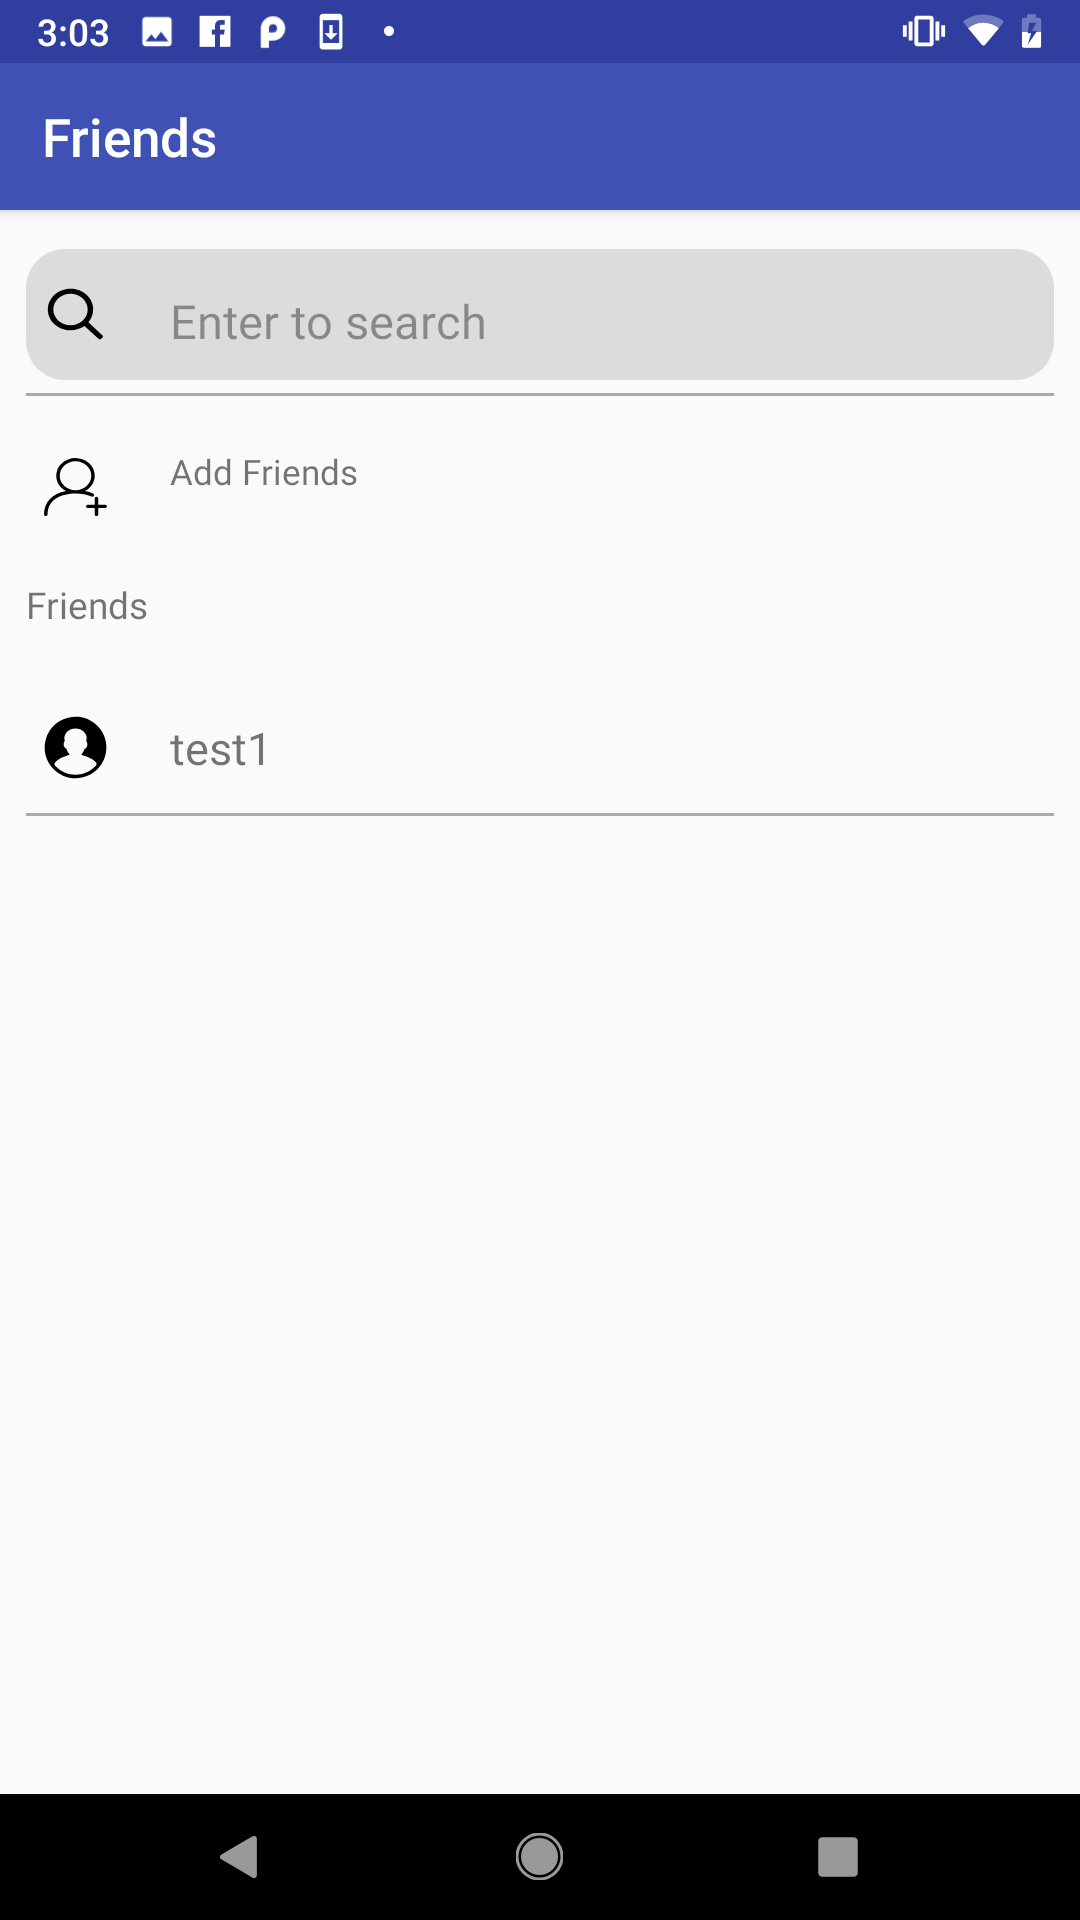
\includegraphics[width=.95\textwidth]{section03/assets/FriendsList.png}
\subcaption{\label{FriendsListUI}}
\end{minipage}%
\begin{minipage}[t]{0.45\textwidth}
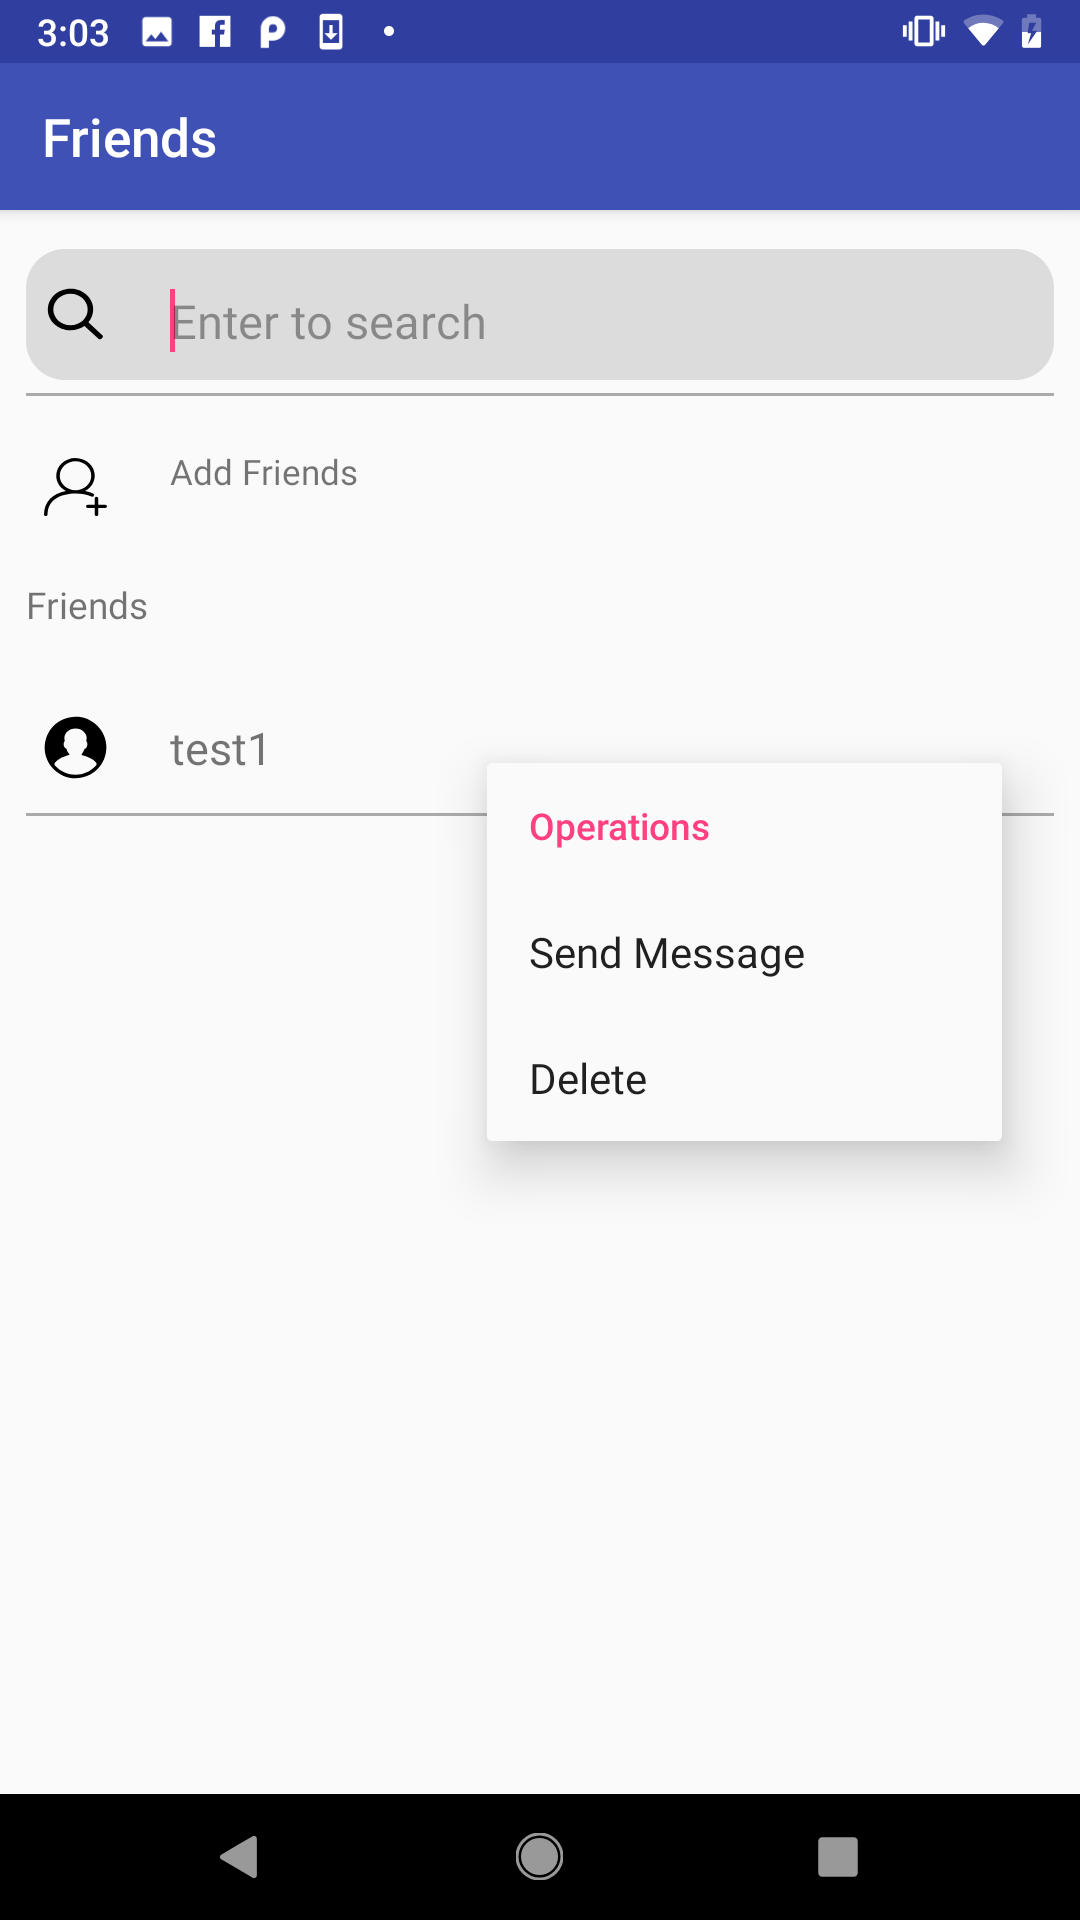
\includegraphics[width=.95\textwidth]{section03/assets/FriendsListAction.png}
\subcaption{\label{FriendsListActionUI}}
\end{minipage}%
\caption[Friends List Page]{\label{WholeFriendsListUI}Friends List Page}
\end{figure}

\textbf{Send Gift Page}

\par After a user chooses to send a gift to one of their friends, they will see the \bsq{Send Gift} page shown in Figure \ref{SendGiftUI}. They open their camera, capture an image, and then select a region of that image which will contain the gift they are sending.  They can choose any four sided shape like trapezoids, rectangles or parallelograms for the region they would like in which they would attach the gift. When they finish region selection, they will see the gift options at the bottom. Users can choose a gift from a pre-defined library of gifts that is included with the application.  In addition, users are able to create their own gifts by taking a picture themselves. 

\begin{figure}[H]
\centering
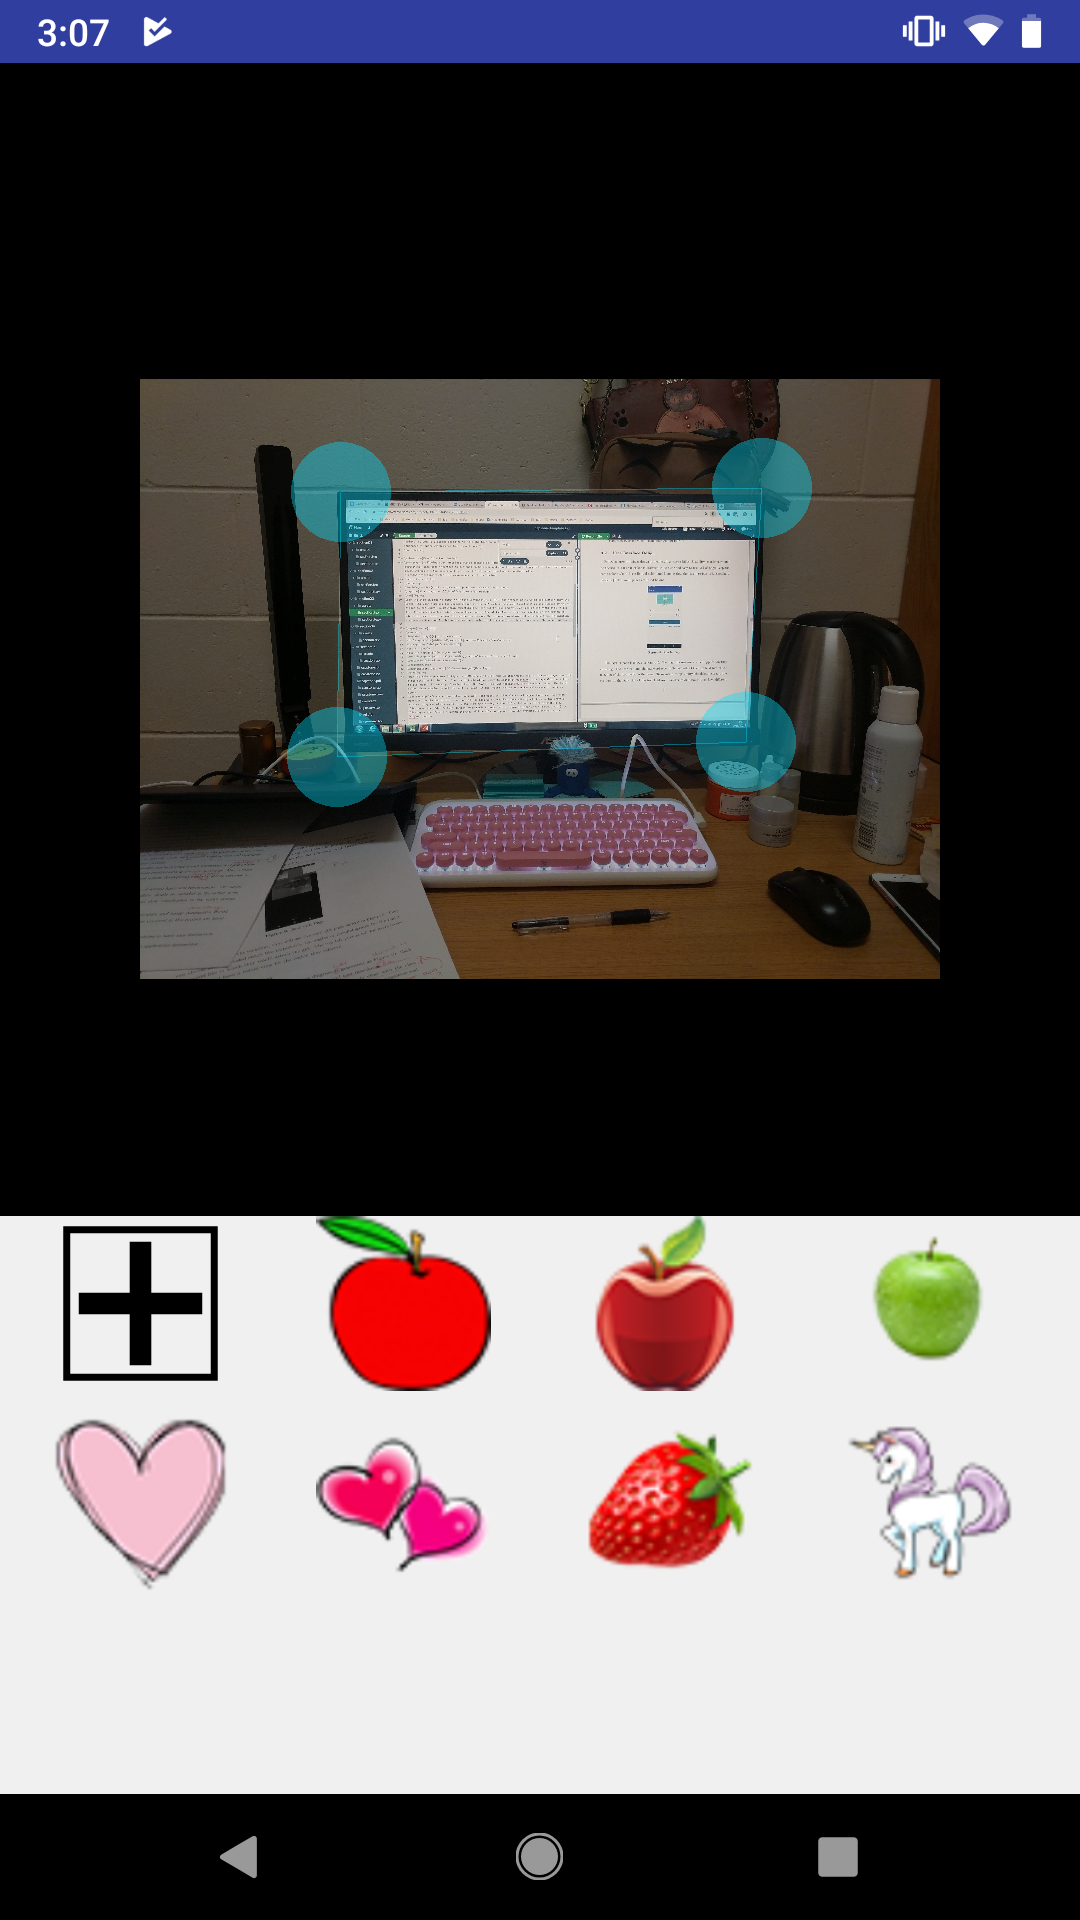
\includegraphics[width=.45\textwidth]{section03/assets/SendGift.png}
\caption[Send Gift Page]{\label{SendGiftUI}Send Gift Page}
\end{figure}

\textbf{Navigation Page}

\par When a user receives a gift, they will see a map view in which the location of the gift will be marked in red and the users location will be marked in blue.  Figure \ref{Navigation} shows an example of this page. Users can use this page to navigate to the location of the gift in order to receive it.

\begin{figure}[H]
\centering
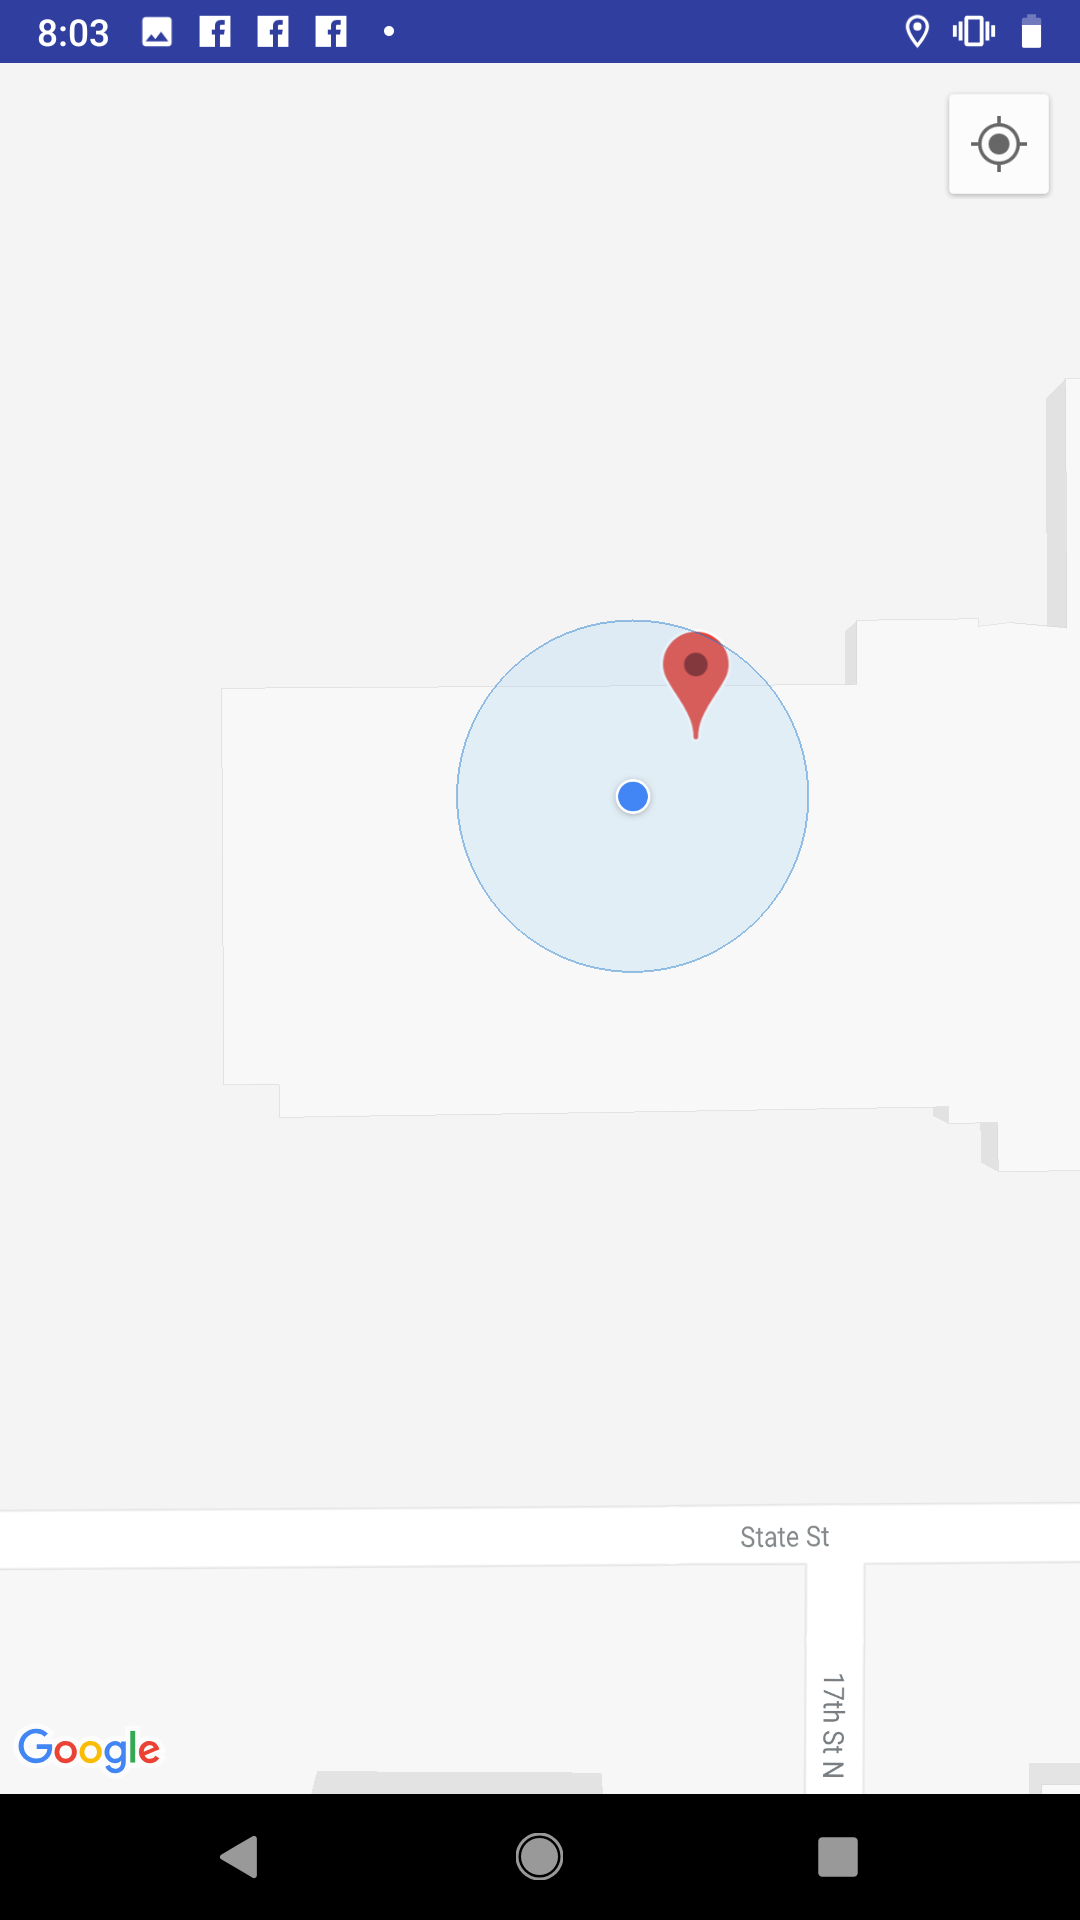
\includegraphics[width=.45\textwidth]{section03/assets/Navigation.png}
\caption[Navigation Page]{\label{Navigation}Navigation Page}
\end{figure}

\subsubsection{The Web User Interface Design}
\paragraph{} The web interface is mainly used to retrieve data from the database and show them in a user readable way. So we designed the web interface as shown in Figure \ref{ViewGift} and Figure \ref{AddFriends}.
\begin{figure}[htb]
\centering
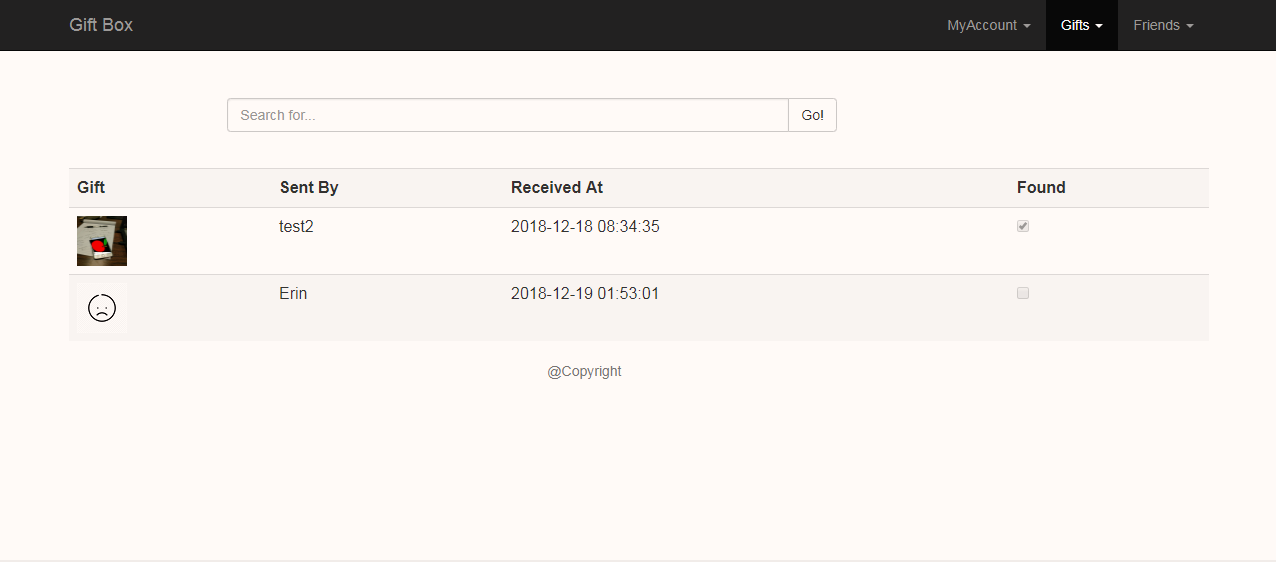
\includegraphics[width=.9\textwidth]{section03/assets/ViewGifts.png}
\caption[View Gift Page for Web Interface]{\label{ViewGift}View Gift Page for Web Interface}
\end{figure}
\par The view gift page is designed similarly to the \bsq{gifts list page} in Android so that there is consistency between the two applications. In Figure \ref{ViewGift} View Gift Page, users will only be able to see those gifts which they have found and an unhappy face in the gift column will be displayed if the gift is not found. Users can also search their gifts list by the username of the sender.

\begin{figure}[htb]
\centering
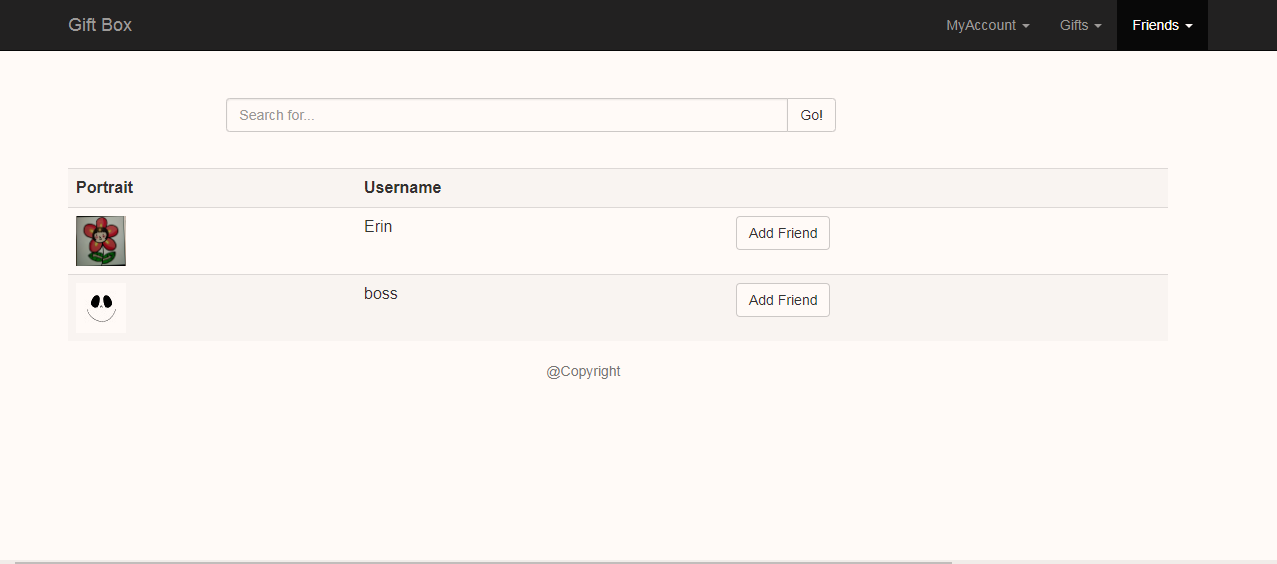
\includegraphics[width=.9\textwidth]{section03/assets/AddFriends.png}
\caption[Add Friend Page for Web Interface]{\label{AddFriends}Add Friend Page for Web Interface}
\end{figure}
\par As shown in Figure \ref{AddFriends} Add Friend Page, all the users which are not currently friends will be listed. Users can also search by username. 


\subsection{Architecture Design}

\paragraph{}This application consists of two components: the Android application and the web application.  The Android application uses Java as the primary language while the web application uses a Tomcat server with a Java/JSP backend.  This section will describe the overall class structure for both the Android and web applications.

\subsubsection{Android Design}
\paragraph{}Based on the functional requirements, the class diagram for the Android application was generated as shown in Figure \ref{AndroidClassDiagram}. Each class corresponds to one or more functional requirements and user interfaces.
\par As we can see, the basic user interaction related activities such as \bsq{log in}, \bsq{log out}, \bsq{edit profile} and so don't have too many algorithm-related functions. We chose a meaningful name which can quickly shows the purpose of the method, so we don't need any illustration for them. We are just going to explain activities and functions about image recognition and navigation.

\begin{figure}[htb]
\centering
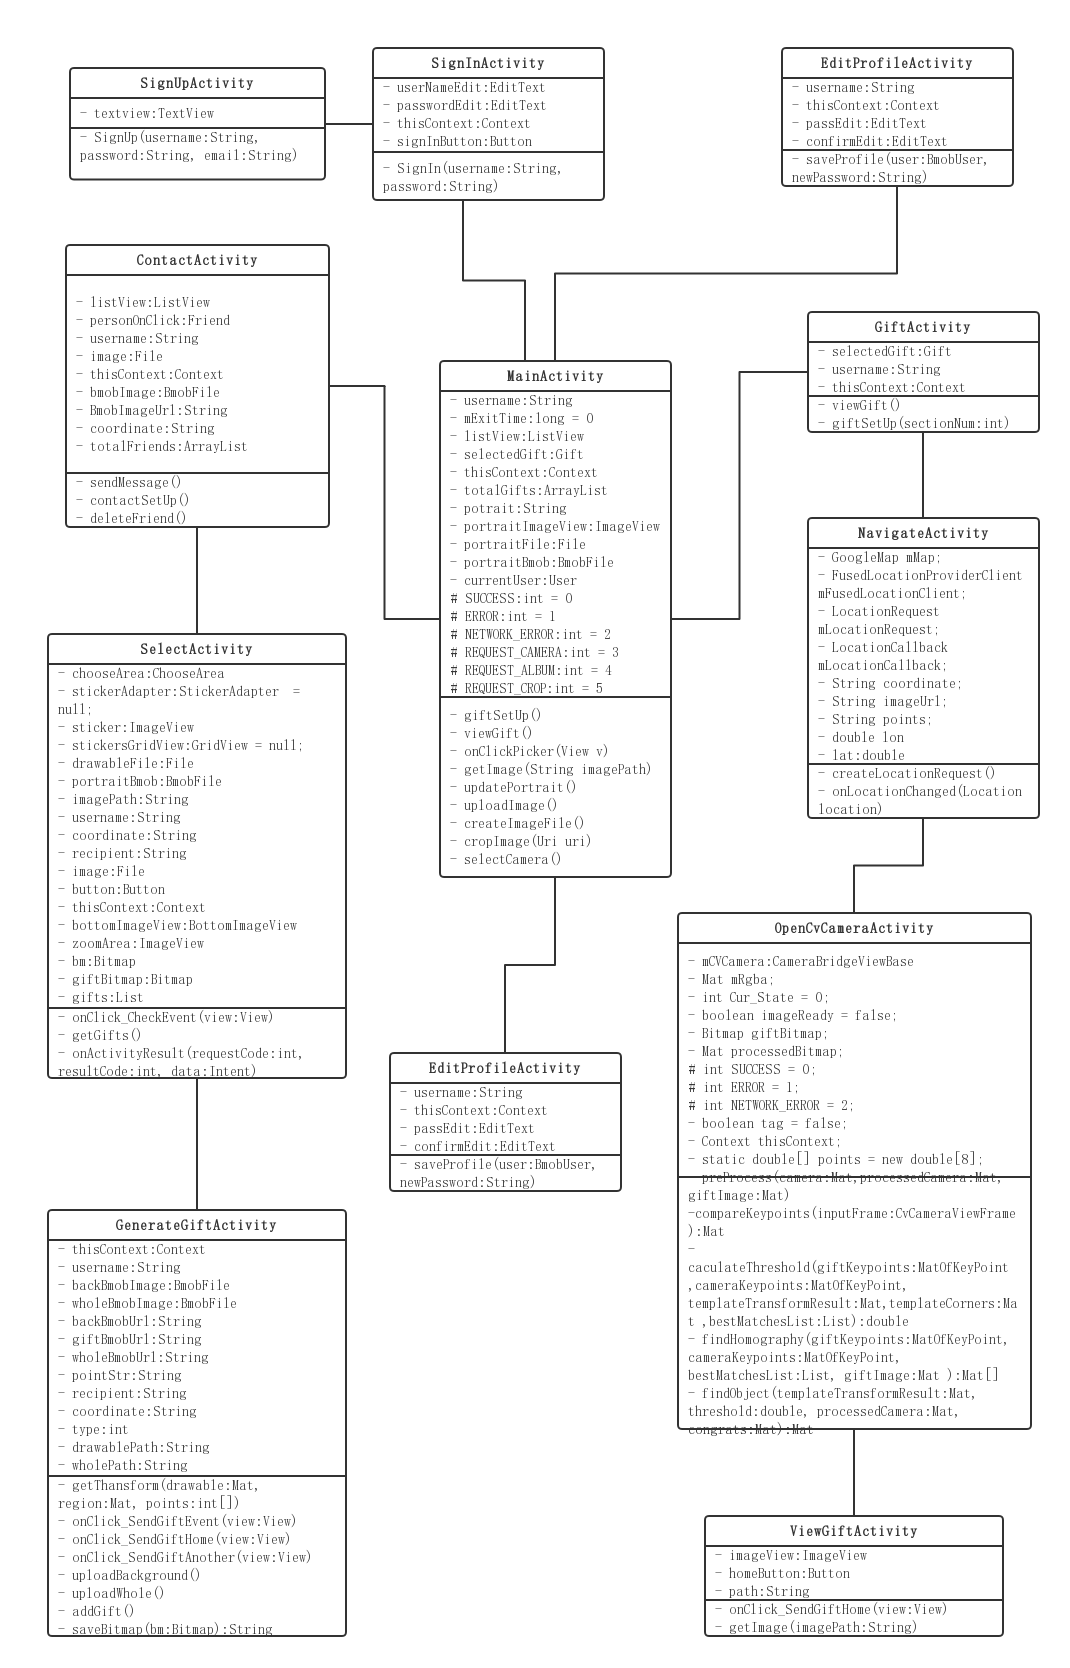
\includegraphics[width=0.8\textwidth]{section03/assets/AndroidClassDiagram.png}
\caption[Class Diagram for Android Application]{\label{AndroidClassDiagram}Class Diagram for Android Application}
\end{figure}

\par The \bsq{ContactActivity} is mainly related to the user interface shown in Figure \ref{FriendsListUI}, users will be able select a recipient and the information will be taken to \bsq{SelectActivity} by an intent and then the system camera will be called to get the background image. The \bsq{chooseArea} attribute is an instance of helper class \bsq{ChooseArea} to let the users choose the region. After that, the gift will fit in the region by \bsq{getTransform} method and \bsq{addGift} method will save all the information to the database.
\par The receiving process is explained as followed. The \bsq{GiftActivity} is designed to show the gift list which is shown in Figure \ref{GiftsListUI}, when users click on a not found gift they will go to \bsq{NavigationActivity}. The \bsq{NavigationActivity} is designed to manage user locations and Google Map activities. Users will be able to see their location on the map and the gift location will be marked as a red point. When users find where the gift is located, the real-time image recognition will start. The camera-captured images will compare with the database saved background image. The \bsq{preProcess} method is used to download the database saved background image and resize the camera-captured images. The \bsq{compareKeypoints} method calculates the keypoints in two images and finds the matches. The \bsq{findHomography} method will use the matches found before to generate the homography and perform a perspective transformation on the template image to correct the image to get the region in camera image. But this method cannot always get the correct result, so the \bsq{caculateThreshold} method calculates the value of the number of keypoints not in the selected region divided by the number of keypoints in detected region, this value will be later used as a threshold to determine if the region we found is good. At last, the \bsq{findObject} method will get the final detected region and show the gift on it.

\subsubsection{Web Application Design}
\begin{figure}[htb]
\centering
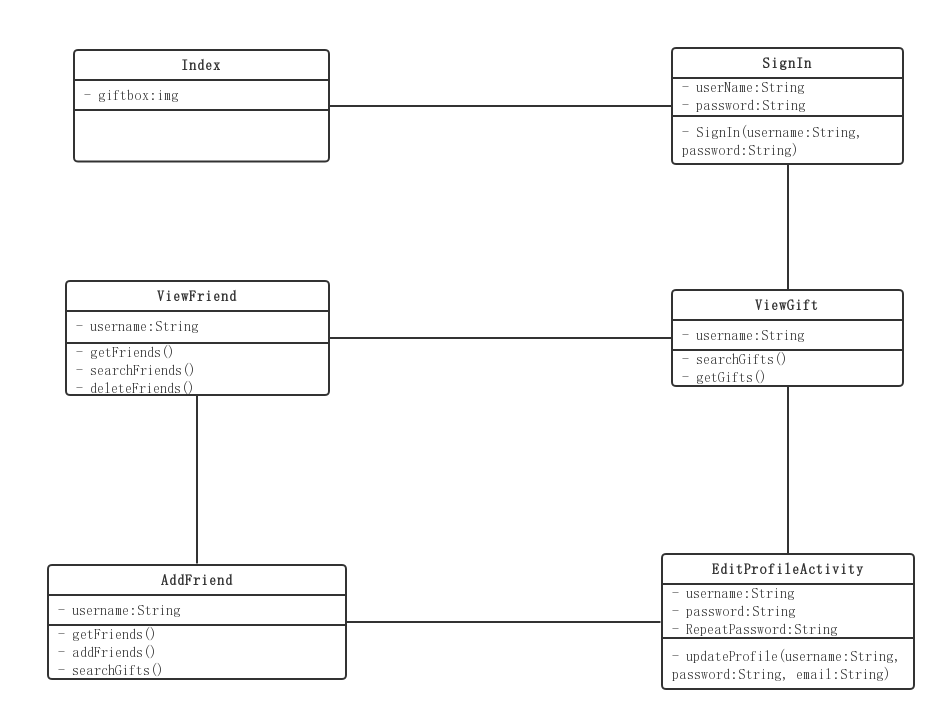
\includegraphics[width=1\textwidth]{section03/assets/WebClassDiagram.png}
\caption[Class Diagram for Web Interface]{\label{WebClassDiagram}Class Diagram for Web Interface}
\end{figure}
\paragraph{} The design and implementation of the web interface is very similar to the Android application. The class diagram for the web interface is shown in Figure \ref{WebClassDiagram}. The \bsq{AddFriends} class is related to Figure \ref{AddFriends} Add Friends Page. In this page, the user will be able to see all the users which are not currently friends. Users are allowed to search for other users by username in this page as well. The \bsq{ViewFriends} class allows users to view their friends list and to delete friends by clicking on the \bsq{delete} button. The \bsq{ViewGifts} class is related to Figure \ref{ViewGift} View Gift Page which allows users to view their received gifts. Users will only be able to see the found gifts and those gifts that have not been found will be replaced by a smiling face. The username attribute in all fields maintains the current user's username. 
